\documentclass[a4paper, 12pt]{article}
\usepackage{vntex}
\usepackage{a4wide,amssymb,epsfig,latexsym,array,hhline,fancyhdr}
\usepackage[normalem]{ulem}
\usepackage[makeroom]{cancel}
\usepackage{amsmath}
\usepackage{amsthm}
\usepackage{multicol,longtable,amscd}
\usepackage{diagbox}%Make diagonal lines in tables
\usepackage{booktabs}
\usepackage{alltt}
\usepackage[framemethod=tikz]{mdframed}% For highlighting paragraph backgrounds
\usepackage{caption,subcaption}
\usepackage{lastpage}
\usepackage[lined,boxed,commentsnumbered]{algorithm2e}
\usepackage{enumerate}
\usepackage{color}
\usepackage{xcolor}
\usepackage{graphicx}							% Standard graphics package
\usepackage{array}
\usepackage{tabularx, caption}
\usepackage{multirow}
\usepackage{multicol}
\usepackage{rotating}
\usepackage{graphics}
\usepackage{geometry}
\usepackage{setspace}
\usepackage{epsfig}
\usepackage{tikz}
\usepackage{listings}
\usepackage{float}
\usetikzlibrary{arrows,snakes,backgrounds}
\usepackage{hyperref}
\hypersetup{urlcolor=black,linkcolor=black,citecolor=black,colorlinks=true} 
%\usepackage{pstcol} 								% PSTricks with the standard color package

\newtheorem{theorem}{{\bf Theorem}}
\newtheorem{property}{{\bf Property}}
\newtheorem{proposition}{{\bf Proposition}}
\newtheorem{corollary}[proposition]{{\bf Corollary}}
\newtheorem{lemma}[proposition]{{\bf Lemma}}

\AtBeginDocument{\renewcommand*\contentsname{Mục lục}}
\AtBeginDocument{\renewcommand*\refname{Tài liệu tham khảo}}
\AtBeginDocument{\renewcommand*\listfigurename{Tiêu đề ảnh}}
%\usepackage{fancyhdr}
\setlength{\headheight}{40pt}
\pagestyle{fancy}
\fancyhead{} % clear all header fields
\fancyhead[L]{
 \begin{tabular}{rl}
    \begin{picture}(25,15)(0,0)
    \put(0,-8){
\includegraphics[width=8mm, height=8mm]{hcmut.png}}
   \end{picture}&
	\begin{tabular}{l}
		\textbf{\bf \ttfamily Trường Đại Học Bách Khoa Tp.Hồ Chí Minh}\\
		\textbf{\bf \ttfamily Khoa Khoa Học \& Kỹ Thuật Máy Tính}
	\end{tabular} 	
 \end{tabular}
}
\fancyhead[R]{
	\begin{tabular}{l}
		\tiny \bf \\
		\tiny \bf 
	\end{tabular}  }
\fancyfoot{} % clear all footer fields
\fancyfoot[L]{\scriptsize \ttfamily Báo cáo môn Kiểm tra phần mềm - Học kì 241}
\fancyfoot[R]{\scriptsize \ttfamily Trang {\thepage}/\pageref{LastPage}}
\renewcommand{\headrulewidth}{0.3pt}
\renewcommand{\footrulewidth}{0.3pt}


%%%
\setcounter{secnumdepth}{4}
\setcounter{tocdepth}{3}
\makeatletter
\newcounter {subsubsubsection}[subsubsection]
\renewcommand\thesubsubsubsection{\thesubsubsection .\@alph\c@subsubsubsection}
\newcommand\subsubsubsection{\@startsection{subsubsubsection}{4}{\z@}%
                                     {-3.25ex\@plus -1ex \@minus -.2ex}%
                                     {1.5ex \@plus .2ex}%
                                     {\normalfont\normalsize\bfseries}}
\newcommand*\l@subsubsubsection{\@dottedtocline{3}{10.0em}{4.1em}}
\newcommand*{\subsubsubsectionmark}[1]{}
%\renewcommand{\thesubsubsection}{\alph{subsubsection}}
\everymath{\color{blue}}
\makeatother

\begin{document}

\begin{titlepage}
\begin{center}
VIETNAM NATIONAL UNIVERSITY, HO CHI MINH CITY \\
UNIVERSITY OF TECHNOLOGY \\
FACULTY OF COMPUTER SCIENCE AND ENGINEERING
\end{center}
\vspace{1cm}

\begin{figure}[h!]
\begin{center}

\includegraphics[width=3cm]{hcmut.png}
\end{center}
\end{figure}

\vspace{1cm}


\begin{center}
\begin{tabular}{c}
\multicolumn{1}{l}{\textbf{{\Large KIỂM TRA PHẦN MỀM (CO3015)}}}\\

~~\\
\hline
\\
\\
\textbf{{\Huge BTL 2: BLACK BOX TESTING}}\\
\\

\\
\hline
\end{tabular}
\end{center}

\vspace{3cm}

\begin{table}[h]
\begin{tabular}{rrl}
\hspace{3 cm} & Giảng viên hướng dẫn: & Bùi Hoài Thắng\\

& Sinh viên thực hiện:
& Phạm Đức Hào - 2111128\\
&& Hồ Trọng Nhân - 2111899\\
&& Đậu Đức Quân - 2114531\\
&& Nguyễn Phúc Minh Quân - 2110479\\
&& Trần Mậu Thật - 2112342
\end{tabular}
\end{table}

\begin{center}
{\footnotesize HO CHI MINH CITY, NOVEMBER 2024}
\end{center}
\end{titlepage}


\newpage
\tableofcontents
\newpage
\section{Giới thiệu:}

\section{Phân công}
 \begin{table}[H]
\centering
\begin{tabular}{|p{3cm}|p{3cm}|l|c|}
\hline 
Reviewer &
Validator &
  \multicolumn{1}{c|}{Feature} &Contributon \\ \hline
Đậu Đức Quân & Trần Mậu Thật &&\\\hline
Hồ Trọng Nhân & Đậu Đức Quân &&\\ \hline
Nguyễn Phúc Minh Quân & Hồ Trọng Nhân &&\\ \hline
Phạm Đức Hào & Nguyễn Phúc Minh Quân &&\\ \hline
Trần Mậu Thật & Phạm Đức Hào &&\\ \hline
\end{tabular}
\caption{Bảng phân công công việc}
\label{tab:my-table}
\end{table}





\newpage
\section{Quá trình làm việc nhóm:}
\subsection{Buổi họp trao đổi những thắc mắc của các thành viên về bài tập lớn và phân công công việc. (15/11/2024)}
Nội dung chính:
\begin{itemize}
    \item
\end{itemize}
Kết quả cuộc họp:
\begin{itemize}
  \item
\end{itemize}

\newpage

\section{Kết quả kiểm thử}

\subsection{Tính năng 1}
\subsubsection{Mô tả}
\subsubsection{Test case}
\subsection{Tính năng 2}

\subsection{Chức năng Tạo sự kiện (Create event)}
\subsubsection{Use case}
\begin{table}[H]
    \centering
    \begin{tabular}{|l|p{11cm}|}
        \hline
        Category & Description \\
        \hline
        Use case name & Create event\\
        \hline
        Actor & Manager \\
        \hline
        Assumption & Người dùng ở trang \url{https://sandbox.moodledemo.net/}. Ngôn ngữ trang web được chỉnh tiếng Việt. Người dùng đăng nhập thành công dưới bất kì tài khoản nào. Người dùng đang ở trang "Bảng điều khiển". \\
        \hline
        Normal flow & 1. Người dùng nhấn vào nút "Sự kiện mới". \\
        & 2. Hệ thống hiển thị bảng "Sự kiện mới". \\
        & 3. Người dùng nhập thông tin có thể bao gồm chữ, số và kí tự vào ô "Tên sự kiện". \\
        & 4. Người dùng chọn thông tin ngày, tháng, năm, giờ, phút của sự kiện. \\
        & 5. Người dùng chọn "Thành viên" hoặc "Hệ thống" tại hàng "Loại sự kiện".\\
        & 6. Người dùng nhấn vào nút "Lưu". \\
        & 7. Hệ thống đóng bảng "Sự kiện mới". \\
        \hline
        Alternative flows & A1. Tại bước 6: \\
        & 6.1. Người dùng nhấn vào nút "Show more". \\
        & 6.2. Người dùng nhập thông tin vào ô "Mô tả". \\
        & Quay lại bước 6 trên Normal flow. \\
        & \\
        & A2. Tại bước 6: \\
        & 6.1. Người dùng nhấn vào nút "Show more". \\
        & 6.2. Người dùng nhập thông tin vào ô "Địa chỉ". \\
        & Quay lại bước 6 trên Normal flow. \\
        & \\
        & A3. Tại bước 6: \\
        & 6.1. Người dùng nhấn vào nút "Show more". \\
        & 6.2. Người dùng chọn lựa chọn "Tới" tại hàng "Thời lượng". \\
        & 6.3. Người dùng chọn thông tin ngày, tháng, năm, giờ, phút kết thúc của sự kiện. \\
        & Quay lại bước 6 trên Normal flow. \\
        & \\
        & A4. Tại bước 6: \\
        & 6.1. Người dùng nhấn vào nút "Show more". \\
        & 6.2. Người dùng chọn lựa chọn "Thời lượng tính bằng phút" tại hàng "Thời lượng". \\
        & 6.3. Người dùng nhập thông tin vào ô dưới "Thời lượng tính bằng phút". \\
        & Quay lại bước 6 trên Normal flow. \\
        & \\
        & A5. Tại bước 6: \\
        & 6.1. Người dùng nhấn vào nút "Show more". \\
        & 6.2. Người dùng chọn vào ô "Lặp lại sự kiện này". \\
        & 6.3. Người dùng nhập thông tin vào ô "Lặp lại hàng tuần, tạo ra tất cả". \\
        & Quay lại bước 6 trên Normal flow. \\
        & \\
        & A6. Tại bước 5: \\
        & 5.1. Người dùng chọn "Mục" tại hàng "Loại sự kiện". \\
        & 5.2. Người dùng chọn các mục cần thiết tại hàng "Mục". \\
        & Quay lại bước 6 trên Normal flow. \\
        \hline
        Exception flows & \\
        & E1. Tại bước 3: \\
        & 3.1. Người dùng không nhập vào ô "Tên sự kiện". \\
        & Thực hiện tiếp tục bước 3 trên Normal flow. Sau khi thực hiện đến bước 6, hệ thống sẽ hiển thị lỗi "Bắt buộc". \\ 
        & Quay lại bước 3 trên Normal flow. \\
        & \\
        & E2. Tại bước A3.6.3: \\
        & 6.3. Người dùng chọn thông tin ngày, tháng, năm, giờ, phút kết thúc của sự kiện diễn ra trước thời điểm bắt đầu. \\
        & Thực hiện tiếp tục bước 6 trên Normal flow. Sau khi thực hiện bước 6, hệ thống báo lỗi "Khoảng thời gian ngày và giờ bạn chọn diễn ra trước khi sự kiện bắt đầu. Vui lòng điều chỉnh trước khi tiếp tục.". \\
        & E3. Tại bước A4.6.3: \\
        & 6.3. Người dùng nhập thông tin không phải số nguyên dương vào ô dưới "Thời lượng tính bằng phút". \\
        & Thực hiện tiếp tục bước 6 trên Normal flow. Sau khi thực hiện bước 6, hệ thống báo lỗi "Khoảng thời gian tính bằng phút mà bạn vừa nhập không có hiệu lực. Vui lòng nhập một khoảng thời gian tính bằng phút lớn hơn 0 hoặc không chọn thời gian.". \\
        & Quay lại bước 6.2 trên Alternative flow A4. \\
        & \\
        & Quay lại bước 6.3 trên Alternative flow A3. \\
        & \\
        E4. Tại bước A6.5.2: \\
        & 5.2. Người dùng xóa hết các mục tại hàng "Mục". \\
        & Thực hiện tiếp tục bước 6 trên Normal flow. Sau khi thực hiện bước 6, hệ thống báo lỗi "Hãy chọn một chuyên mục". \\
        & Quay lại bước 5.2 trên Alternative flow A6. \\
        \hline
    \end{tabular}
    \caption{Use case: Create event}
    \label{Use case: Create event}
\end{table}
\subsubsection{Activity diagram}
\begin{figure}[H]
    \centering
    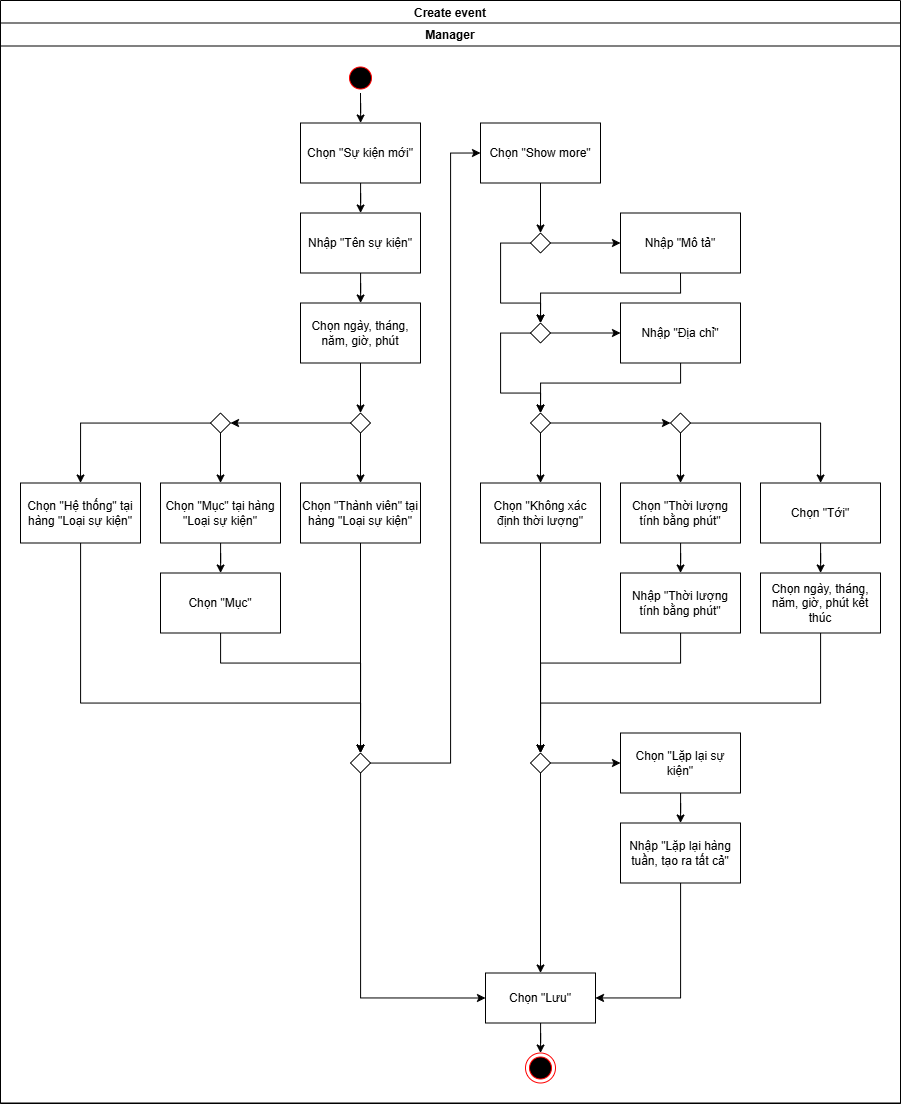
\includegraphics[height=0.5\textheight]{images/ce-action.drawio.png}
    % \caption{Caption}
    \label{fig:enter-label}
\end{figure}
\subsubsection{Sử dụng phương pháp Boundary value analysis để kiểm thử}
Kiểm tra giá trị biên cho thời lượng, thời điểm kết thúc sự kiện. Ta có các ràng buộc:
\begin{itemize}
    \item 0 < Thời lượng
    \item Thời điểm bắt đầu sự kiện > Thời điểm kết thúc sự kiện
\end{itemize}
Vì 2 giá trị thời lượng và thời điểm kết thúc sự kiện không thể tồn tại đòng thời. Ta có các bảng test case cho phương pháp Robust Boundary Value:
\begin{table}[H]
    \centering
    \begin{tabular}{|c|c|c|}
        \hline
        ID TC & Thời lượng & Expected \\
        \hline
        CE-002-001 & 0 & Khoảng thời gian tính ... \\
        \hline
        CE-002-002 & 9999 & Thêm sự kiện thành công. \\
        \hline
        CE-002-003 & 999999999999999999 & Thêm sự kiện thành công. \\
        % Không viết được vào CSDL
        \hline
    \end{tabular}
    \caption{Test case cho Thời lượng - Robust Boundary Value}
    \label{tab:my_label}
\end{table}
\begin{table}[H]
    \centering
    \begin{tabular}{|c|p{3cm}|p{3cm}|p{4cm}|}
        \hline
        ID TC & Thời điểm bắt đầu sự kiện & Thời điểm kết thúc sự kiện &  Expected \\
        \hline
        CE-002-004 & 20/11/2024 19:00 & 20/11/2024 18:59 & Khoảng thời gian ngày....\\
        \hline
        CE-002-005 & 20/11/2024 19:00 & 21/11/2024 18:59 & Thêm sự kiện thành công. \\
        \hline
    \end{tabular}
    \caption{Test case cho Thời điểm kết thúc sự kiện - Robust Boundary Value}
    \label{tab:my_label}
\end{table}
% \subsubsection{Sử dụng phương pháp Equivalence class partitioning}
% \subsubsection{Sử dụng phương pháp Decision table để kiểm thử}
\subsubsection{Sử dụng phương pháp Use-case testing để kiểm thử}
Dựa vào use case và activity diagram, ta có các đường kiểm thử:
\begin{itemize}
    \item 1 -> 2 -> 3 -> 4 -> 5 -> 6 -> 7
    \item 1 -> 2 -> 3 -> 4 -> 5 -> A1.6.1 -> A1.6.2 -> 6 -> 7
    \item 1 -> 2 -> 3 -> 4 -> 5 -> A2.6.1 -> A2.6.2 -> 6 -> 7
    \item 1 -> 2 -> 3 -> 4 -> 5 -> A3.6.1 -> A3.6.2 -> A3.6.3 -> 6 -> 7
    \item 1 -> 2 -> 3 -> 4 -> 5 -> A4.6.1 -> A4.6.2 -> A4.6.3 -> 6 -> 7
    \item 1 -> 2 -> 3 -> 4 -> 5 -> A5.6.1 -> A5.6.2 -> A5.6.3 -> 6 -> 7
    \item 1 -> 2 -> 3 -> 4 -> A6.5.1 -> A6.5.2 -> 6 -> 7
    \item 1 -> 2 -> E1.3.1 -> 4 -> 5 -> 6
    \item 1 -> 2 -> 3 -> 4 -> 5 -> A3.6.1 -> A3.6.2 -> E2.6.3 -> 6
    \item 1 -> 2 -> 3 -> 4 -> 5 -> A4.6.1 -> A4.6.2 -> E3.6.3 -> 6
    \item 1 -> 2 -> 3 -> 4 -> A6.5.1 -> E4.5.2 -> 6
\end{itemize}
Các test case và thực hiện kiểm thử trong file excel (có id dạng CE-001-0xx).
\subsection{Chức năng Đổi mật khẩu (Change password)}
\subsubsection{Use case}
\begin{table}[H]
    \centering
    \begin{tabular}{|l|p{11cm}|}
        \hline
        Category & Description \\
        \hline
        Use case name & Change password \\
        \hline
        Actor & Người dùng \\
        \hline
        Assumption & Người dùng ở trang \url{https://sandbox.moodledemo.net/}. Ngôn ngữ trang web được chỉnh tiếng Việt. Người dùng đăng nhập thành công dưới bất kì tài khoản nào. Người dùng đang ở trang "Trang chủ". \\
        \hline
        Normal flow & 1. Người dùng nhấn vào nút mũi tên góc phải trên ngay bên cạnh hình đại diện. \\
        & 2. Người dùng nhấn vào "Tùy chọn". \\
        & 3. Người dùng nhấn vào "Đổi mật khẩu". \\
        & 4. Người dùng nhập đúng mật khẩu hiện tại vào ô "Mật khẩu hiện hành".\\
        & 5. Người dùng nhập mật khẩu mới có thể bao gồm cả chữ, số, kí tự và khác với mật khẩu hiện hành vào ô "Mật khẩu mới".\\
        & 6. Người dùng nhập chính xác thông tin đã nhập ở ô "Mật khẩu mới" vào ô "Mật khẩu mới (lại)".\\
        & 7. Người dùng nhấn vào nút "Lưu những thay đổi". \\
        & 8. Hệ thống hiển thị "Mật khẩu đã được thay đổi". \\
        \hline
        Alternative flows & Không có. \\
        \hline
        Exception flows & E1. Tại bước 4: \\
        & 4.1. Người dùng không nhập thông tin ở nội dung "Mật khẩu hiện hành". \\ 
        & Thực hiện tiếp tục bước 5 trên Normal flow. Sau khi thực hiện bước 7, hệ thống sẽ hiển thị lỗi "Bắt buộc". \\
        & Quay lại bước 4 trên Normal flow. \\
        & \\
        & E2. Tại bước 5: \\
        & 5.1. Người dùng không nhập thông tin ở nội dung "Mật khẩu mới". \\
        & Thực hiện tiếp tục bước 6 trên Normal flow. Sau khi thực hiện bước 7, hệ thống sẽ hiển thị lỗi "Bắt buộc". \\
        & Quay lại bước 5 trên Normal flow. \\
        & \\
        & E3. Tại bước 6: \\
        & 6.1. Người dùng không nhập thông tin ở nội dung "Mật khẩu mới (lại)". \\
        & Thực hiện tiếp tục bước 7 trên Normal flow. Sau khi thực hiện bước 7, hệ thống sẽ hiển thị lỗi "Bắt buộc". \\
        & Quay lại bước 6 trên Normal flow. \\
        & \\
        & E4. Tại bước 4: \\
        & 4.1. Người dùng nhập nhập thông tin tại ô "Mật khẩu hiện hành" chưa chính xác. \\
        & Thực hiện tiếp tục bước 5 trên Normal flow. Sau khi thực hiện bước 7, hệ thống sẽ hiển thị lỗi "Đăng nhập sai, xin vui lòng thử lại". \\
        & Quay lại bước 4 trên Normal flow. \\
        & \\
        & E5. Tại bước 6: \\
        & 6.1. Người dùng nhập nhập thông tin tại ô "Mật khẩu mới (lại)" chưa khớp với nội dung đã nhập tại ô "Mật khẩu mới". \\
        & Thực hiện tiếp tục bước 7 trên Normal flow. Sau khi thực hiện bước 7, hệ thống sẽ hiển thị lỗi "Các mật khẩu không trùng khớp". \\
        & Quay lại bước 5 trên Normal flow. \\
        & \\
        & E6. Tại bước 5: \\
        & 5.1. Người dùng nhập mật khẩu mới giống với nội dung mật khẩu hiện tại vào ô "Mật khẩu mới". \\
        & Thực hiện tiếp tục bước 6 trên Normal flow. Sau khi thực hiện buốc 7, hệ thống sẽ hiển thị lỗi "Mật khẩu mới phải khác mật khẩu hiện hành". \\
        & Quay lại bước 5 trên Normal flow. \\
        \hline
    \end{tabular}
    \caption{Use case: Change password}
    \label{Use case: Change password}
\end{table}
\subsubsection{Activity diagram}
\begin{figure}[H]
    \centering
    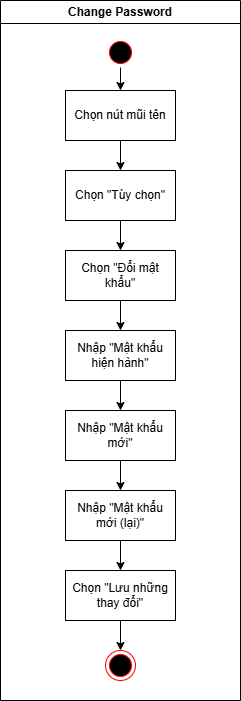
\includegraphics[height=0.5\textheight]{images/cp-action.drawio.png}
    % \caption{Caption}
    \label{fig:enter-label}
\end{figure}
% \subsubsection{Sử dụng phương pháp Boundary value analysis để kiểm thử}
\subsubsection{Sử dụng phương pháp Equivalence class partitioning}
Ta có các nhóm giá trị cho "Mật khẩu hiện hành", "Mật khẩu mới" và "Mật khẩu mới (lại)".
\begin{itemize}
    \item Mật khẩu hiện hành
    \begin{itemize}
        \item C1: không trùng với mật khẩu hiện tại (invalid)
        \item C2: trùng với mật khẩu hiện tại (valid)
    \end{itemize}
    \item Mật khẩu mới
    \begin{itemize}
        \item N1: trùng với mật khẩu hiện tại (invalid)
        \item N2: không trùng với mật khẩu hiện tại (valid)
    \end{itemize}
    \item Mật khẩu mới (lại)
    \begin{itemize}
        \item R1: không trùng với mật khẩu mới (invalid)
        \item R2: trùng với mật khẩu mới (valid)
    \end{itemize}
\end{itemize}
Bảng testcase:
\begin{table}[H]
    \centering
    \begin{tabular}{|c|p{2cm}|p{2cm}|p{2cm}|p{4cm}|}
        \hline
        ID TC & Mật khẩu hiện hành & Mật khẩu mới & Mật khẩu mới (lại) & Expected \\
        \hline
        CP-003-001 & sandbox24 & a & a & Thay đổi mật khẩu thành công \\
        \hline
        CP-003-002 & a & b & b & Đăng nhập sai...\\
        \hline
        CP-003-003 & sandbox24 & sandbox24 & sandbox24 & Mật khẩu mới... \\
        \hline
        CP-003-004 & sandbox24 & a & b & Các mật khẩu...\\
        \hline
    \end{tabular}
    \label{tab:my_label}
\end{table}
\subsubsection{Sử dụng phương pháp Decision table để kiểm thử}
Ta có các điều kiện:
\begin{enumerate}
    \item Nếu "Mật khẩu hiện hành" chính xác.
    \item Nếu "Mật khẩu mới" không trùng với mật khẩu hiện tại.
    \item Nếu "Mật khẩu mới (lại)" trùng với "Mật khẩu mới".
\end{enumerate}
Ta có các action:
\begin{enumerate}
    \item Thay đổi mật khẩu thành công.
    \item Hiện lỗi "Đăng nhập sai, xin vui lòng thử lại".
    \item Hiện lỗi "Mật khẩu mới phải khác mật khẩu hiện hành".
    \item Hiện lỗi "Các mật khẩu không trùng khớp".
\end{enumerate}
Decision table:
\begin{table}[H]
    \centering
    \begin{tabular}{|c|c|c|c|}
        \hline
        Stub & Rule 1 & Rule 2 & Rule 3 \\
        \hline
        1 & T & T & T \\
        \hline
        2 & F & x & x \\
        \hline
        3 & T & F & x \\
        \hline
        4 & T & T & F \\
        \hline
    \end{tabular}
    % \caption{Caption}
    \label{tab:my_label}
\end{table}
Từ decision table, ta có các test case tương tự test case cho giải pháp Equivalence class partitioning.
\subsubsection{Sử dụng phương pháp Use-case testing để kiểm thử}
Dựa vào usecase và activity diagram, ta có các đường cần kiểm thử:
\begin{itemize}
    \item 1 -> 2 -> 3 -> 4 -> 5 -> 6 -> 7 -> 8
    \item 1 -> 2 -> 3 -> E1.4.1 -> 5 -> 6 -> 7
    \item 1 -> 2 -> 3 -> 4 -> E2.5.1 -> 6 -> 7
    \item 1 -> 2 -> 3 -> 4 -> 5 -> E3.6.1 -> 7
    \item 1 -> 2 -> 3 -> E4.4.1 -> 5 -> 6 -> 7
    \item 1 -> 2 -> 3 -> 4 -> 5 -> E5.6.1 -> 7
    \item 1 -> 2 -> 3 -> 4 -> E6.5.1 -> 7-> 7
\end{itemize}
Các test case và thực hiện kiểm thử trong file excel (có id dạng CP-001-0xx).
\section{Tổng kết}
\end{document}
